%%%%%%%%%%%%%%%%%%%%%%%%%%%%%%%%%%%%%%%%%
% Short Sectioned Assignment
% LaTeX Template
% Version 1.0 (5/5/12)
%
% This template has been downloaded from:
% http://www.LaTeXTemplates.com
%
% Original author:
% Frits Wenneker (http://www.howtotex.com)
%
% License:
% CC BY-NC-SA 3.0 (http://creativecommons.org/licenses/by-nc-sa/3.0/)
%
%%%%%%%%%%%%%%%%%%%%%%%%%%%%%%%%%%%%%%%%%

%----------------------------------------------------------------------------------------
%	PACKAGES AND OTHER DOCUMENT CONFIGURATIONS
%----------------------------------------------------------------------------------------

\documentclass[paper=a4, fontsize=11pt]{scrartcl} % A4 paper and 11pt font size

\usepackage[T1]{fontenc} % Use 8-bit encoding that has 256 glyphs
\usepackage{fourier} % Use the Adobe Utopia font for the document - comment this line to return to the LaTeX default
\usepackage[english]{babel} % English language/hyphenation
\usepackage{amsmath,amsfonts,amsthm} % Math packages

\usepackage{lipsum} % Used for inserting dummy 'Lorem ipsum' text into the template
\usepackage{graphicx}
\usepackage{float}
\usepackage{sectsty} % Allows customizing section commands
\allsectionsfont{ \normalfont\scshape} % Make all sections centered, the default font and small caps

\usepackage{fancyhdr} % Custom headers and footers
\pagestyle{fancyplain} % Makes all pages in the document conform to the custom headers and footers
\fancyhead{} % No page header - if you want one, create it in the same way as the footers below
\fancyfoot[L]{} % Empty left footer
\fancyfoot[C]{} % Empty center footer
\fancyfoot[R]{\thepage} % Page numbering for right footer
\renewcommand{\headrulewidth}{0pt} % Remove header underlines
\renewcommand{\footrulewidth}{0pt} % Remove footer underlines
\setlength{\headheight}{13.6pt} % Customize the height of the header

\numberwithin{equation}{section} % Number equations within sections (i.e. 1.1, 1.2, 2.1, 2.2 instead of 1, 2, 3, 4)
\numberwithin{figure}{section} % Number figures within sections (i.e. 1.1, 1.2, 2.1, 2.2 instead of 1, 2, 3, 4)
\numberwithin{table}{section} % Number tables within sections (i.e. 1.1, 1.2, 2.1, 2.2 instead of 1, 2, 3, 4)

\setlength\parindent{0pt} % Removes all indentation from paragraphs - comment this line for an assignment with lots of text

%----------------------------------------------------------------------------------------
%	TITLE SECTION
%----------------------------------------------------------------------------------------

\newcommand{\horrule}[1]{\rule{\linewidth}{#1}} % Create horizontal rule command with 1 argument of height

\title{	
\normalfont \normalsize 
\textsc{CS 646 - IR} \\ [25pt] % Your university, school and/or department name(s)
\horrule{0.5pt} \\[0.4cm] % Thin top horizontal rule
\huge P1 \\ % The assignment title
\horrule{2pt} \\[0.5cm] % Thick bottom horizontal rule
}

\author{Patrick Verga} % Your name

\date{\normalsize\today} % Today's date or a custom date

\begin{document}

\maketitle % Print the title

%----------------------------------------------------------------------------------------
%	PROBLEM 1
%----------------------------------------------------------------------------------------

\section {Implementation Choices}

I parsed the raw xml using the BeautifulSoup library. I first broke each book into pages and then represented the page as all text within a <line> tag, not including subtags of line which held metadata. I then removed punctuation, converted all text to lowercase, and finally split the page on whitespace.


\section {Runtimes}

\begin{tabular}{ l | c }
Dataset & Runtime (H : MM : S) \\
\hline
  tiny & 0 : 00 : 9.95  \\
  small & 0 : 03 : 21.5  \\
  medium & 0 : 58 : 27.75  \\
  big & 2 : 34 : 24.57  \\
\end{tabular}

\section {Differences in Dataset Statistics}
Even though big was about 30x larger than small, the top words and the probabilities of those words are roughly equivalent. The same is true of medium. The number of unique words does not increase as drastically as the number of total words between the data sets, as shown later in Figure \ref{fig:heap}. 

Having the larger data does however give better special word associations. For example, small has spurious previous word statistics such as handsome church which do not occur in the larger datasets.

\section {Implications For Designing an IR System}
These results show that it does not take an extremely large amount of data to generate relavent statistics about word frequencies. This also demonstrates the importance of things like stop word removal. This also shows the benefit of using idf term weighting for similarity calculations.

\section{Zipf's Law}
Zipf's law has to do with occurances of a word relative to its rank. Zipf's law as to do with occurances of a word relative to its rank. The bulk of the total words is contained in the few top most frequently occuring words. There is also a drastic drop off from rank 1 word to rank 2 to rank 3 etc. 

Zipf's law clearly holds for this data set as shown in \ref{fig:zipf}

\begin{figure}[H] 
\centerline{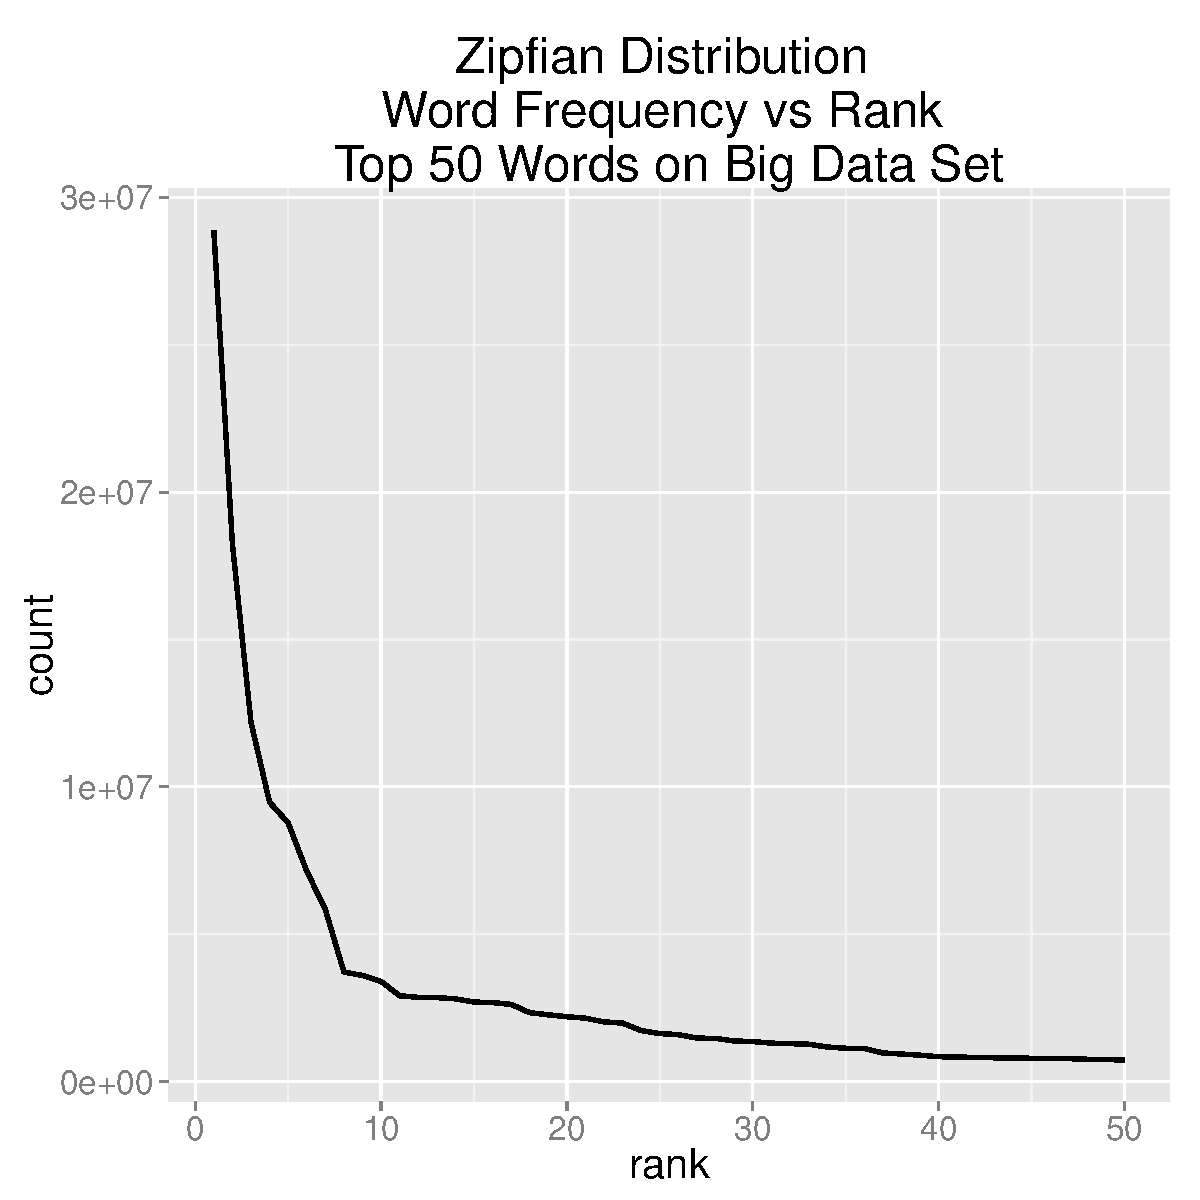
\includegraphics[width=1\textwidth]{zipf-plot}}
  \caption{Here we plot the top 50 most occuring words on the big data set by their count.}
  \label{fig:zipf}
 \end{figure}


\section{Heap's Law}
Heap's law deals with the relation between total words and unique words in a corpus. Initially there is a rapid increase in the number of unique words. However, the increase in unique word drops off quickly as the corpus grows larger. 

It seems like Heap's law may hold for this data, though it is not extremely clear in this plot possibly due to using only 4 datapoints. The plot would have most likely been clearer plotting, for a single data set, the relation between unique and total words as the dataset is processed.

\begin{figure}[H] 
\centerline{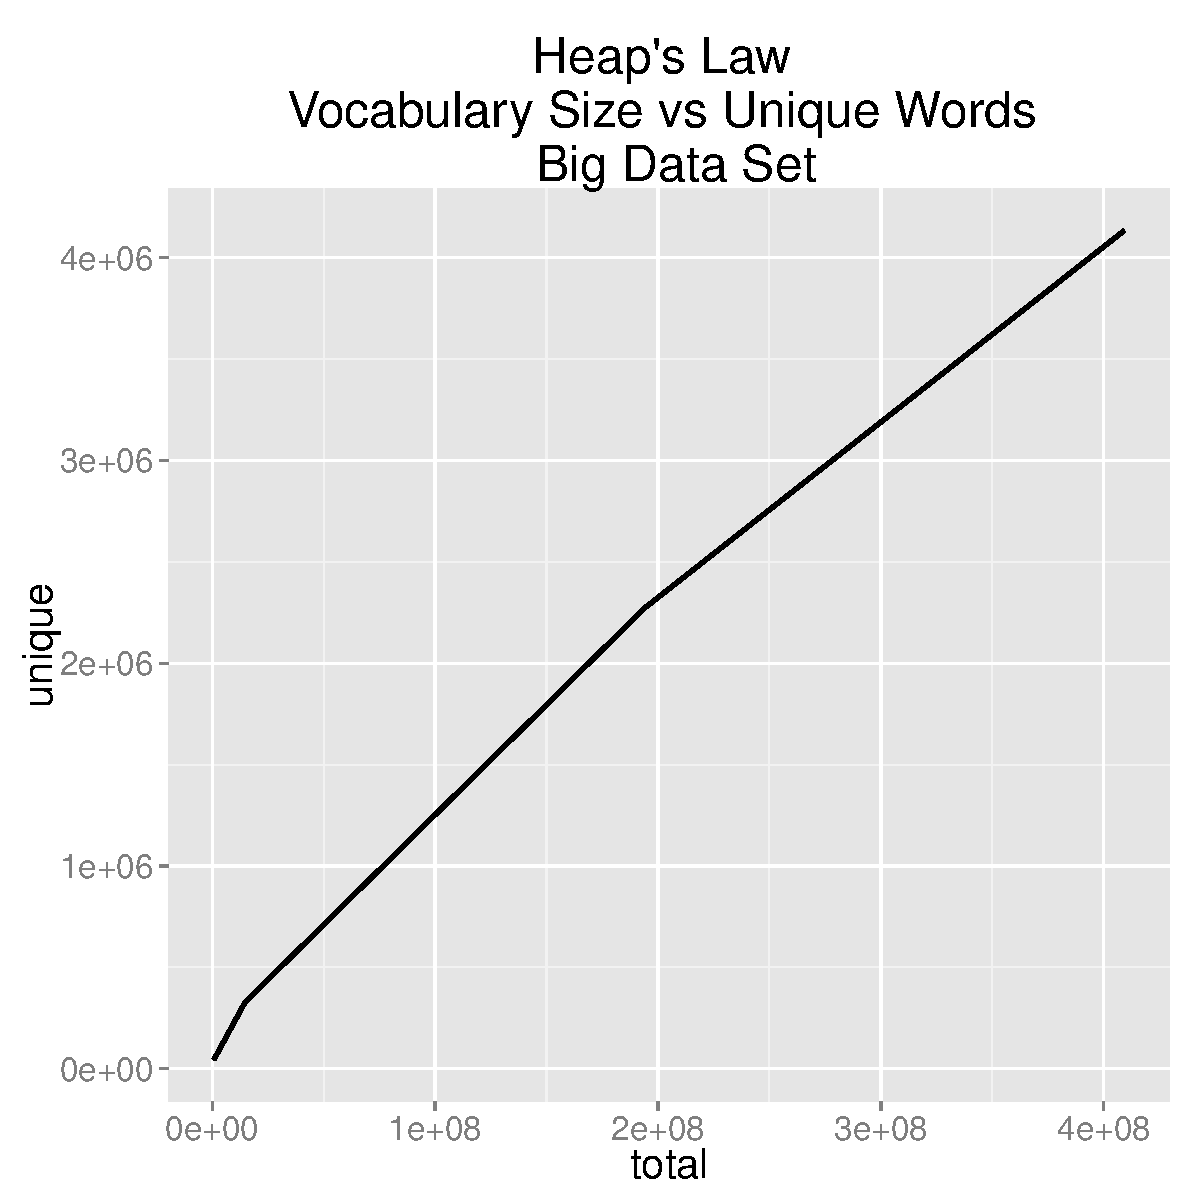
\includegraphics[width=1\textwidth]{heap-plot}}
  \caption{Plotting the total words vs unique words for the 4 data sets: tiny, small, medium, and big. Note the differences in axis size}
  \label{fig:heap}
 \end{figure}


\section{Strong Word Associations}
For this we look at the word following the special word. For example: \textbf{salt} water.

\hspace{-2 cm}
\begin{tabular}{ |l |c | c | c |c |c | c | c| c| c| c|}
Word & Rank 1 & Rank 2 & Rank 3 & Rank 4 & Rank 5 & Rank 6 & Rank 7 & Rank 8 & Rank 9 & Rank 10 \\
\hline
  \textbf{powerful} & than & influence & army & enough & nation & fleet & effect & man & force & party \\
  \textbf{strong} & enough & position & force & man & hand & hold & desire & men & drink & feeling \\
  \textbf{salt} & water & lake & solution & sea & springs & works & fish & meant & marshes & pork \\
  \textbf{butter} & cheese & flies & eggs & fat & made & fly & milk & maker & making & worth \\
\end{tabular}


\section {Words Likely to Follow}
Here we look at the top 5 words likely to follow the 3 special words as well as their entropy: P(w2|w1)

\hspace{-2.65 cm}
\begin{tabular}{| l | c | c | c | c | c |c | c | c | c | c |}
Word & Rank 1 & Ent. 1 & Rank 2 & Ent. 2 & Rank 3 & Ent. 3 & Rank 4 & Ent. 4 & Rank 5 & Ent. 5 \\
\hline
  \textbf{washington} & d & 0.089451 & dc & 0.033986 & city & 0.019926 & county & 0.018546 & george & 0.017597  \\
  \textbf{church} & dedicated & 0.040684 & history & 0.011985 & music & 0.011067 & where & 0.010856 & built & 0.008748  \\
  \textbf{james} & ii & 0.046639 & river & 0.032846 & madison & 0.021453 & g & 0.020119 & monroe & 0.014899 \\
\end{tabular}


\section {Words Likely to Proceed}

Here we look at the top 5 words likely to proceed the 3 special words as well as their entropy: P(w2|w1)

\hspace{-2.8 cm}
\begin{tabular}{| l | c | c | c | c | c |c | c | c | c | c |}
Word & Rank 1 & Ent. 1 & Rank 2 & Ent. 2 & Rank 3 & Ent. 3 & Rank 4 & Ent. 4 & Rank 5 & Ent. 5 \\
\hline
  \textbf{washington} & general & 0.07240 & george & 0.06514 & gen & 0.026457 & fort & 0.02605 & president & 0.01720  \\
  \textbf{church} & parish & 0.05653 & catholic & 0.04256 & presbyterian & 0.034152 & episcopal & 0.03145 & christian & 0.02821  \\
  \textbf{james} & sir & 0.06872 & st & 0.06693 & king & 0.049857 & rev & 0.03045 & mr & 0.02445  \\
\end{tabular}





















\end{document}